

\section{Thesis Overview}
%the most text-heavy of the whole presentation, I promise
\begin{frame}
\frametitle{Thesis overview}
\begin{itemize}
\item Both climate and oceanographic science disciplines are feeling a data explosion and are struggling to scale. 
\item Unprecedented amounts of data are made available by governmental agencies like NOAA and NASA and used by the scientific community to draw inferences about the Earth. 
\item The traditional visualization and delivery tools can be improved to handle the surge of big data. 
\item This presentation describes techniques used to create visualization and data retrieval products. 
\item Global data sets need modern web app technologies for professional and amateur to visualize, retrieve, and analyze data as quickly, accurately, and painlessly as possible.
\end{itemize}
\end{frame}

\begin{frame}
\frametitle{Focus on two data sets}
\begin{columns}
\column{0.5\textwidth}
\begin{figure}
    \centering
    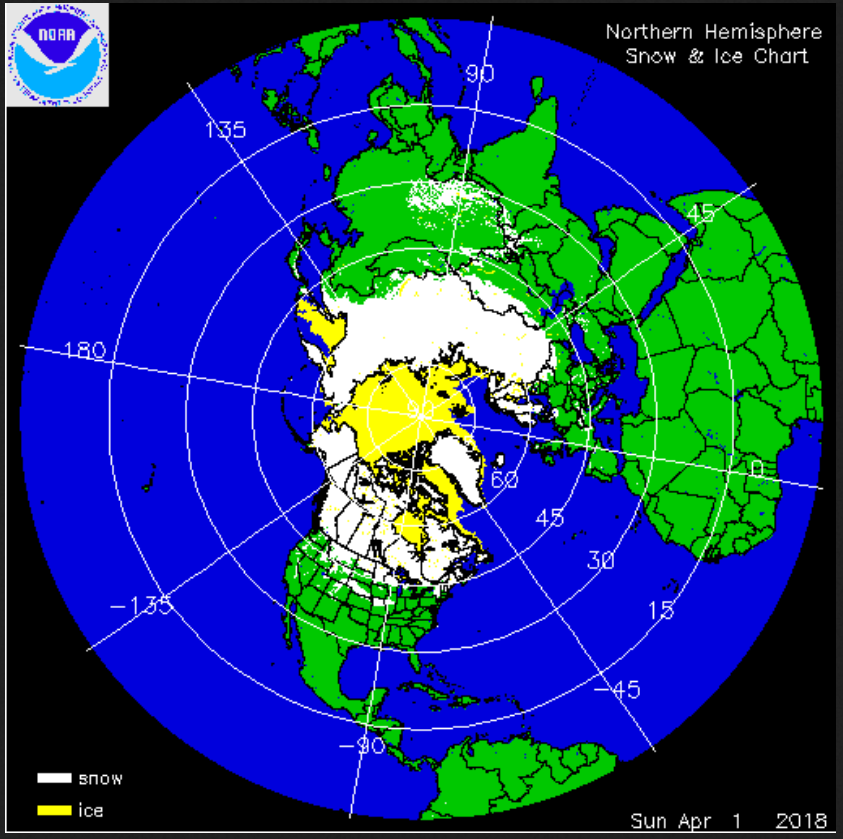
\includegraphics[width=\columnwidth]{nat-ice.png}
    \caption{\tiny{IMS snow cover, \url{http://www.natice.noaa.gov/ims/}}}
\end{figure}
\column{0.5\textwidth}
\begin{figure}
    \centering
    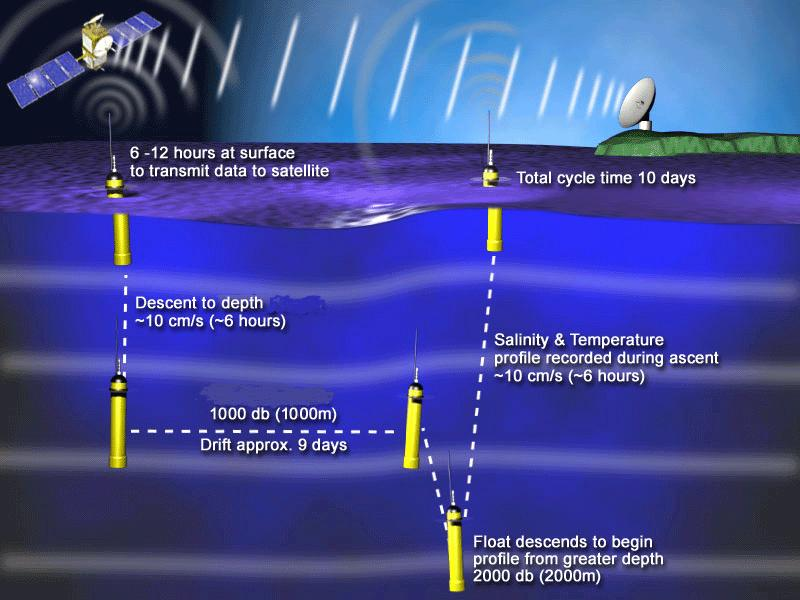
\includegraphics[width=\columnwidth]{operation_park_profile.jpg}
    \caption{\tiny{Detail of one profile cycle \url{http://www.argo.ucsd.edu/How_Argo_floats.html}}}
\end{figure}
\end{columns}
\end{frame}